\documentclass{article}
\usepackage{graphicx}
\usepackage[margin=1in]{geometry} 
\usepackage{float}
\usepackage{xcolor}
\usepackage{hyperref}
\usepackage{float}
 
\begin{document}

\title{Project 4 - Facebook API and Simulator \\ COP5615, Fall 2015}
 
\author{Grant Hernandez and Chelsea Metcalf}
 
\maketitle % this produces the title block
 
\section*{Code Structure}

\subsection*{Client Simulator}

The client simulator is structured to create users (with each having their own actor), pages, and to have users make friends. Once these initial tasks are complete, the user actors begin simulating activity. The structure of the simulator is shown in \autoref{cli-struct}. Based off of a certain ``load factor'' users will post more frequently. This can be thought of as their aggressiveness.

\begin{figure}[H]
  \centering
  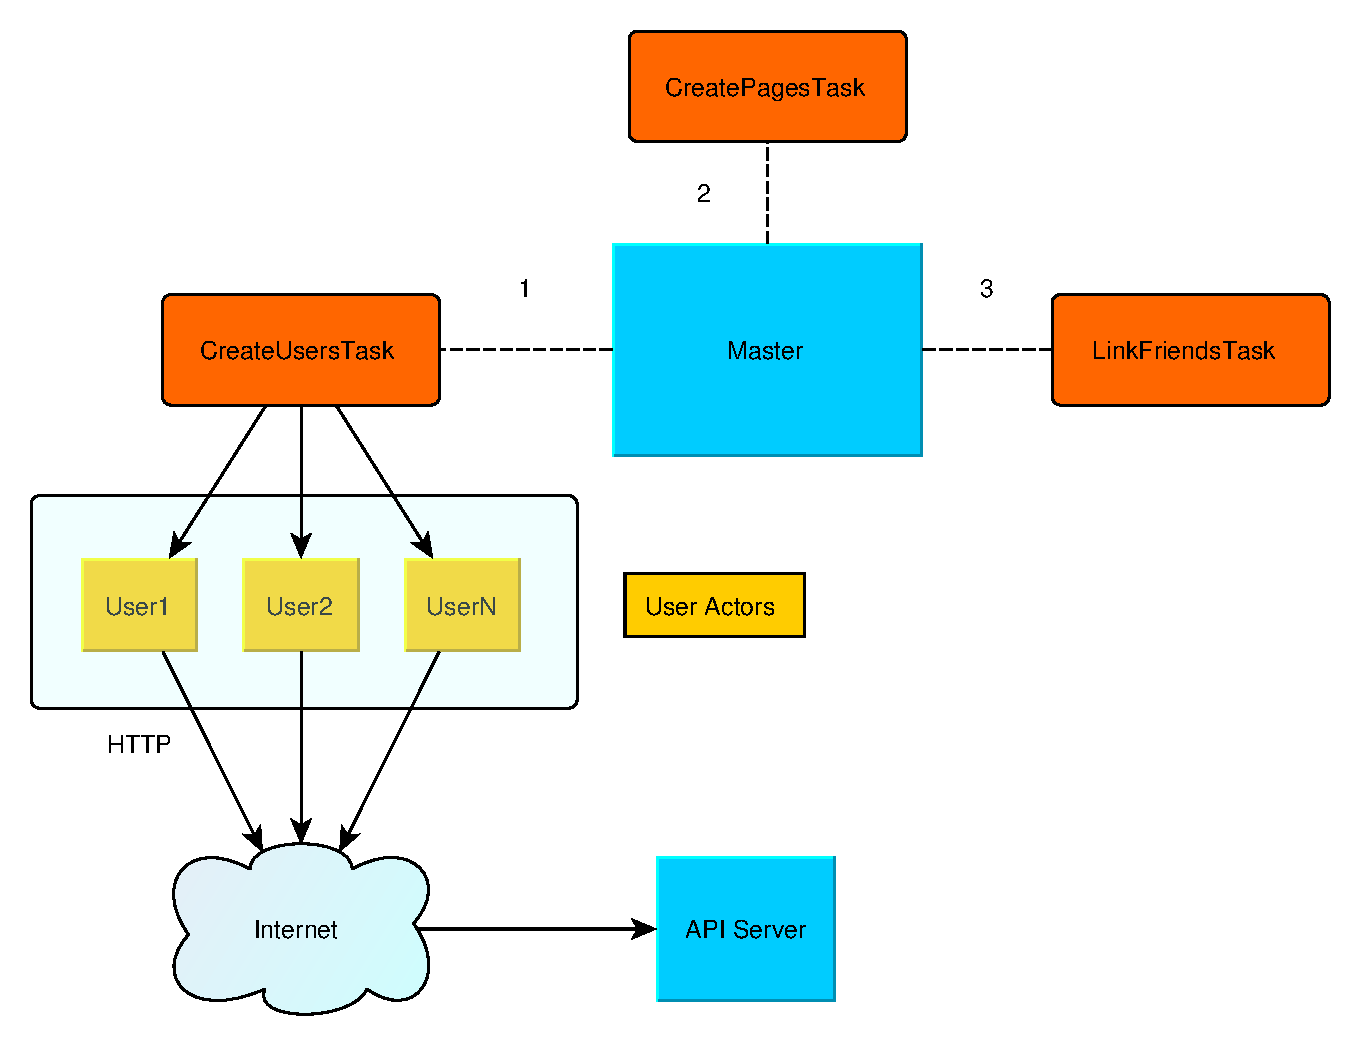
\includegraphics[scale=0.5]{diagrams/client-structure.pdf}
  \caption{Client structure}
  \label{cli-struct}
\end{figure}

\subsection*{API Server}
The API server utilizes Spray to build a REST API using the Spray-routing DSL. In each unique REST route either an entity is deserialized using Spray-JSON or parameters are extracted from the route URI. Once the inputs are extracted, they are passed by message, along with the \texttt{RequestContext} to a data manager Actor. This actor serializes requests to Facebook data objects and implements all of the business logic for the site. This includes creating users, pages, posts, albums, and pictures. It also allows these items to be looked up by ID and retrieved. Additionally, auxiliary functions such as adding friends are implemented here due to the easy data object access. This is shown in \autoref{svr-struct}.

\begin{figure}[H]
  \centering
  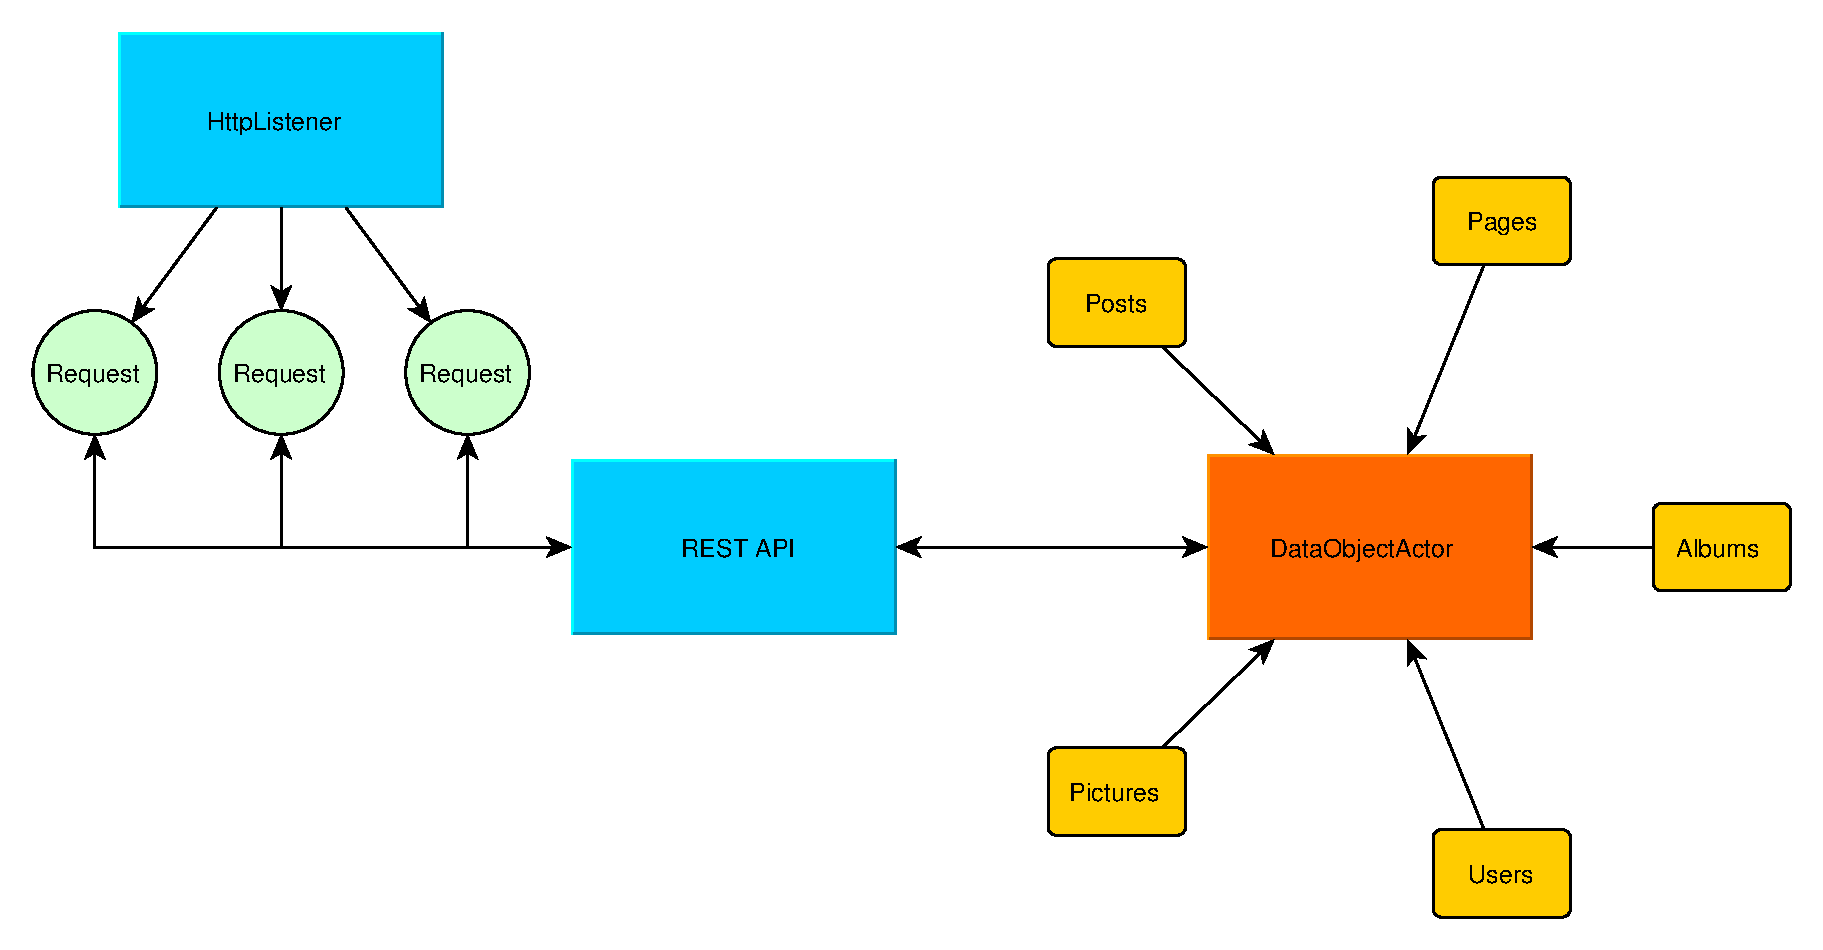
\includegraphics[scale=0.5]{diagrams/server-structure.pdf}
  \caption{Server structure}
  \label{svr-struct}
\end{figure}

One limitation of this approach is that all of the data objects are stored in one Actor instance. This makes programming easy, but since actors are single threaded and can only process one message at a time, this becomes a limitation. A solution to this would be to have a more generic way of storing data such that any Actor could manage a chunk of user data. Then the API frontend would have to message a router to figure out which Actor was responsible for the required objects. This would increase the parallelism of the API server.

For organizing data, all major objects are considered ``entities'' and all derive from a similar base class (\autoref{ents}). This base class holds common attributes such as identifier and modified\_time. For example, UserEnt which holds a user's profile information derives from FacebookEntity. Each specialized Ent has its own JSON serialization and deserialization routines which allow it to be communicated over HTTP.

\begin{figure}[H]
  \centering
  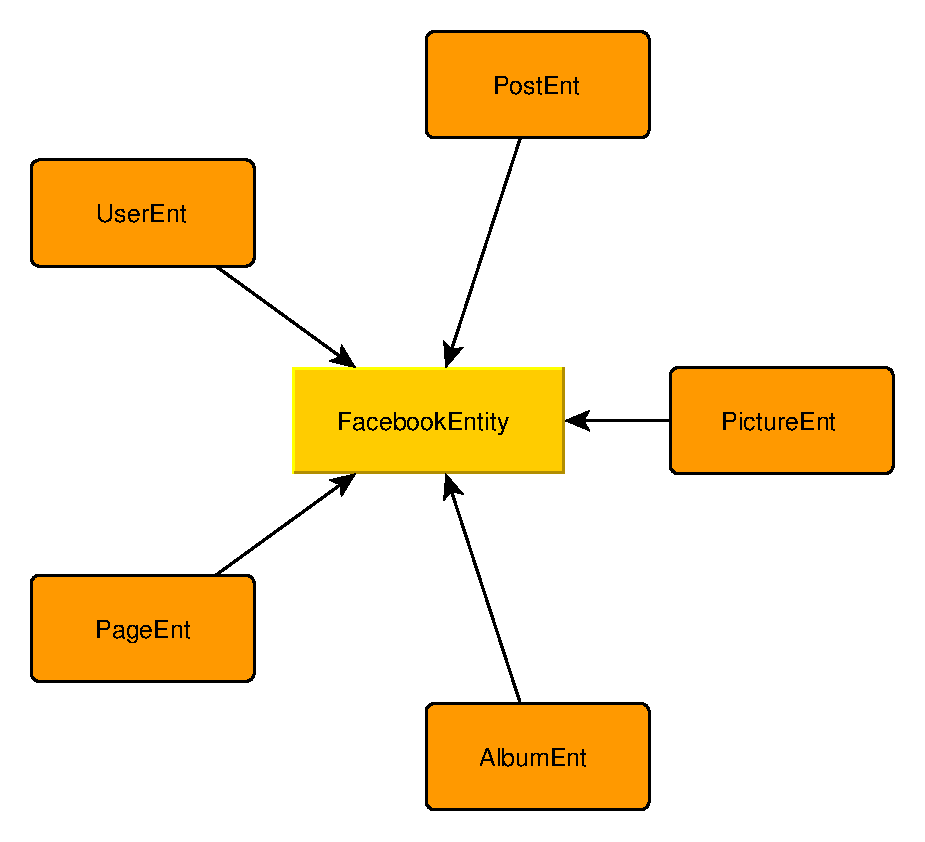
\includegraphics[scale=0.5]{diagrams/entity-hierarchy.pdf}
  \caption{Entity hierarchy}
  \label{ents}
\end{figure}

\section*{REST API}
Below is a simplified table describing the Facebook REST API.

\begin{table}[H]
\centering
\begin{tabular}{|p{1cm}|p{5.5cm}|p{5.5cm}|p{2.53cm}|} 
 \hline
 Verb  & Route & Description  & Body\\ [0.5ex] \hline\hline
 POST  & /user/ & Creates a new user with the parameters & UserCreateForm\\ \hline
 GET & /user/\{user-id\} & Get a user by ID & UserEnt \\ \hline
 POST & /user/\{user-id\}/add\_friend/\{f-id\} & Add a friend from user-id to f-id (friend ID) & TextResult \\ \hline
 GET & /user/\{user-id\}/friends & Get user-id's friends list & Array[Identifier] \\ \hline
 GET & /post/\{post-id\} & Retrieve a post by ID  & PostEnt \\ [1ex] \hline
 POST & /page/ & Creates a new page & PageEnt \\ [1ex] \hline
 GET & /page/{page-id} & Get page by ID & PageEnt \\ [1ex] \hline
 POST & /album/ & Creates a new album & AlbumEnt \\ [1ex] \hline
 GET & /album/{album-id} & Get album by ID & AlbumEnt \\ [1ex] \hline
 POST & /picture/ & Creates a new picture & PictureEnt \\ [1ex] \hline
 GET & /picture/{picture-id} & Get picture by ID & PictureEnt \\ [1ex] \hline
\end{tabular}
\caption{Facebook REST API}
\label{table:api}
\end{table}

There are more API routes in the actual server, but \autoref{table:api} has a good sample of the routes.

\section*{User Studies}
We generated our users based on these user studies. They are a combination of actual Facebook studies and studies on the general population.

\subsection*{Age}
\begin{table}[H]
\centering
\begin{tabular}{|p{2cm}||p{2cm}|} 
 \hline
 Age & Percentage \\ [0.5ex] 
 \hline\hline
 13 - 17 & 0 percent \\
 \hline
 18 - 24 & 15 percent \\
 \hline
 25 - 34 & 29 percent \\
 \hline
 35 - 44 & 24 percent \\ [1ex] 
 \hline
\end{tabular}
\caption{Age Study \cite{sproutsocialwebsite}}
\label{table:1}
\end{table}

\subsection*{Relationship Status}
\begin{table}[H]
\centering
\begin{tabular}{|p{3cm}||p{3cm}|} 
 \hline
 Relationship Status & Percentage \\ [0.5ex] 
 \hline\hline
 Single & 37 percent \\
 \hline
 Married & 31 percent \\
 \hline
 In a Relationship & 24 percent \\
 \hline
 Engaged & 3 percent \\
 \hline
 It's Complicated & 3 percent \\ [1ex] 
 \hline
\end{tabular}
\caption{Relationship Status Study \cite{relstatuswebsite}}
\label{table:2}
\end{table}

\subsection*{Political Affiliation}
\begin{table}[H]
\centering
\begin{tabular}{|p{3cm}||p{3cm}|} 
 \hline
 Party Affiliation & Percentage \\ [0.5ex] 
 \hline\hline
 Republicans & 25 percent \\
 \hline
 Democrats & 29 percent \\
 \hline
 Independents & 41 percent \\ [1ex] 
 \hline
\end{tabular}
\caption{Political Affiliation Study \cite{polstatuswebsite}}
\label{table:3}
\end{table}

\subsection*{Interested In}
\begin{table}[H]
\centering
\begin{tabular}{|p{3cm}||p{3cm}|} 
 \hline
 Interested In & Percentage \\ [0.5ex] 
 \hline\hline
 Straight & 96.6 percent \\
 \hline
 Gay/Lesbian & 2.4 percent \\
 \hline
 Bisexual & 0.7 percent \\ [1ex] 
 \hline
\end{tabular}
\caption{Political Affiliation Study \cite{interestedinwebsite}}
\label{table:4}
\end{table}

\subsection*{Facebook Activity}
\begin{figure}[H]
  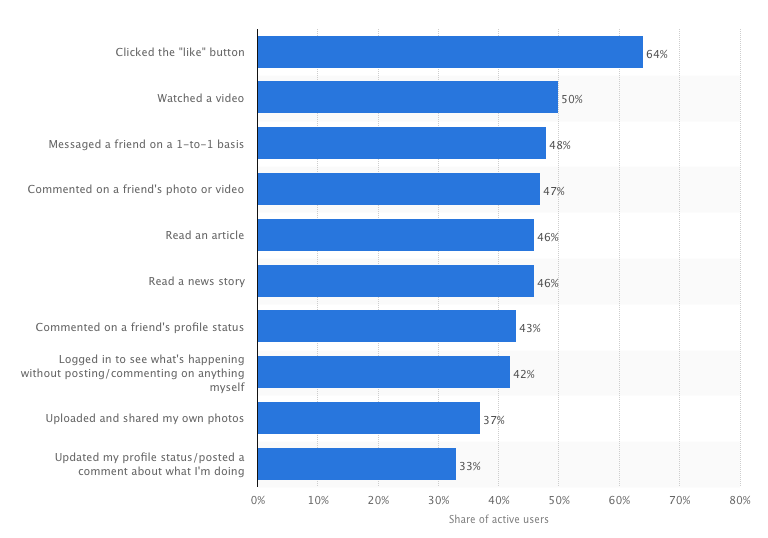
\includegraphics[width=\linewidth]{fbact.png}
  \caption{Percentage of Activity for Facebook Users. \cite{fbactwebsite}}
  \label{fig:fbact}
\end{figure}

Worldwide, there are over 1.49 billion monthly active Facebook users \cite{fbstatswebsite}. In Europe, over 307 million people are on Facebook. On average, the Like and Share buttons are viewed on 10 million websites daily. Five new profiles are created every second, with 76 percent of Facebook users female and 66 percent male. With every minute on Facebook, 510 comments are posted, 293,000 statuses are updated, and 136,000 photos are uploaded. \\

\noindent In a study conducted from 2007 to 2010 \cite{fbstats2website}, the three biggest usage spikes of Facebook occurred on weekdays at 11:00 AM, 3:00 PM, and 8:00 PM. Facebook users are less active on Sundays compared to all days in the week.

\section*{Testing}
For testing, our primary metrics were the number of users simultaneously using the API and the number of sustained API requests per second. To show how the number of requests per second (hereafter r/s) increased, we used 4 clients on separate servers, each managing the same number of users. This means that each client was running the total number of users divided by 4. The plots showing the r/s over time are below.

\begin{figure}[H]
  \centering
  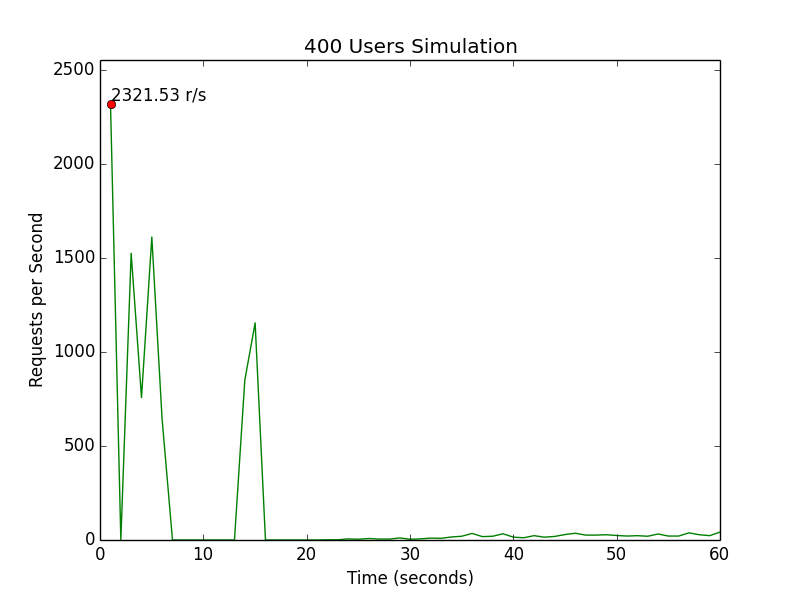
\includegraphics[scale=0.5]{diagrams/rps-400.png}
  \caption{400 user simulation}
  %\label{svr-struct}
\end{figure}

\begin{figure}[H]
  \centering
  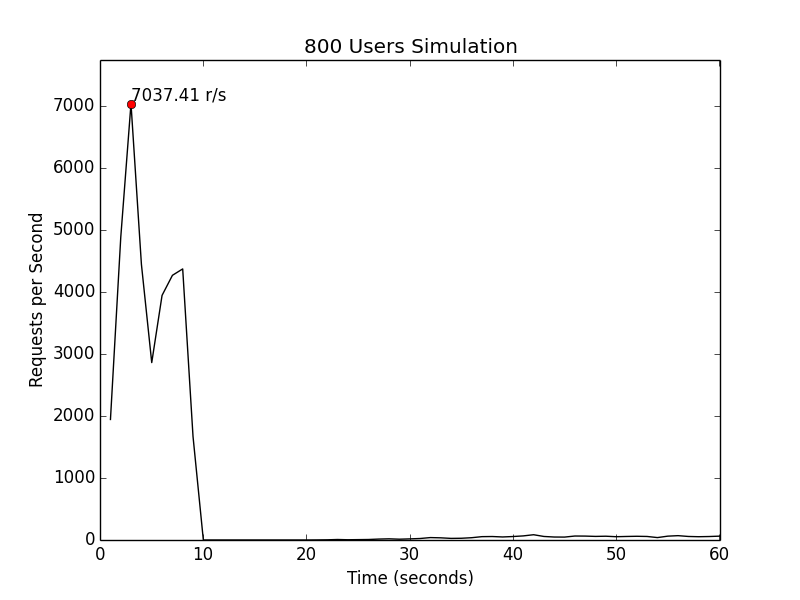
\includegraphics[scale=0.5]{diagrams/rps-800.png}
  \caption{800 user simulation}
  %\label{svr-struct}
\end{figure}

\begin{figure}[H]
  \centering
  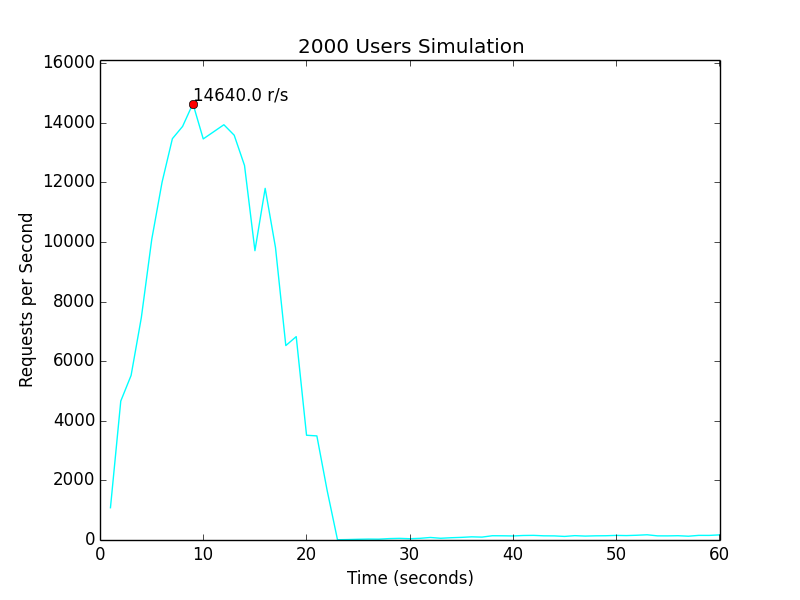
\includegraphics[scale=0.5]{diagrams/rps-2000.png}
  \caption{2000 user simulation}
  %\label{svr-struct}
\end{figure}

\begin{figure}[H]
  \centering
  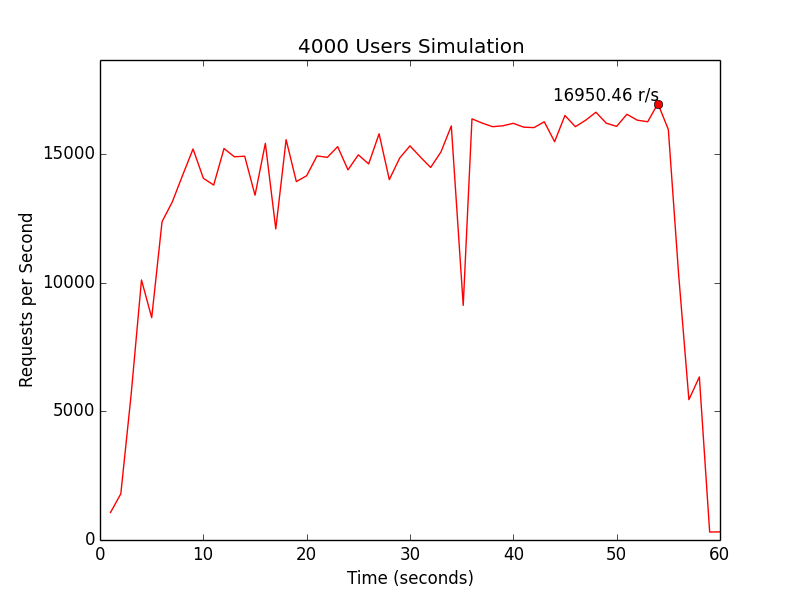
\includegraphics[scale=0.5]{diagrams/rps-4000.png}
  \caption{4000 user simulation}
  %\label{svr-struct}
\end{figure}

\begin{figure}[H]
  \centering
  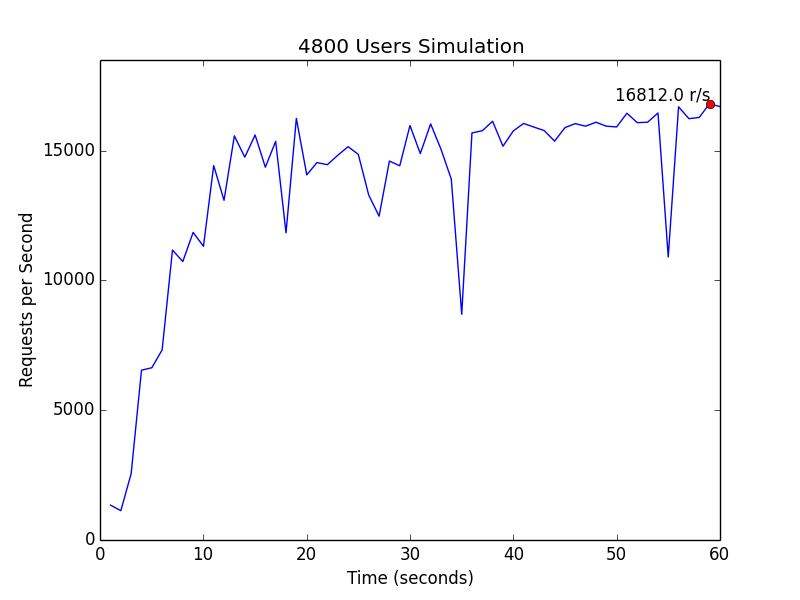
\includegraphics[scale=0.5]{diagrams/rps-4800.png}
  \caption{4800 user simulation}
  %\label{svr-struct}
\end{figure}

\begin{figure}[H]
  \centering
  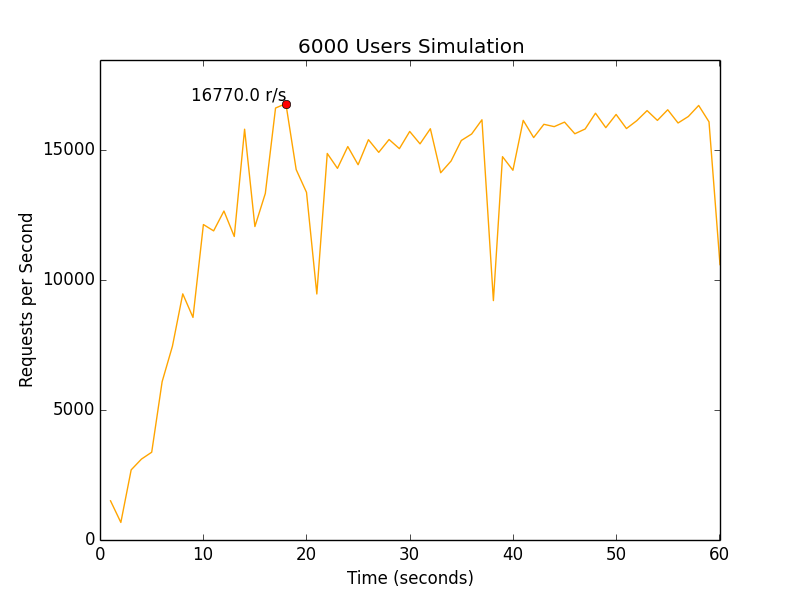
\includegraphics[scale=0.5]{diagrams/rps-6000.png}
  \caption{6000 user simulation}
  %\label{svr-struct}
\end{figure}

\begin{figure}[H]
  \centering
  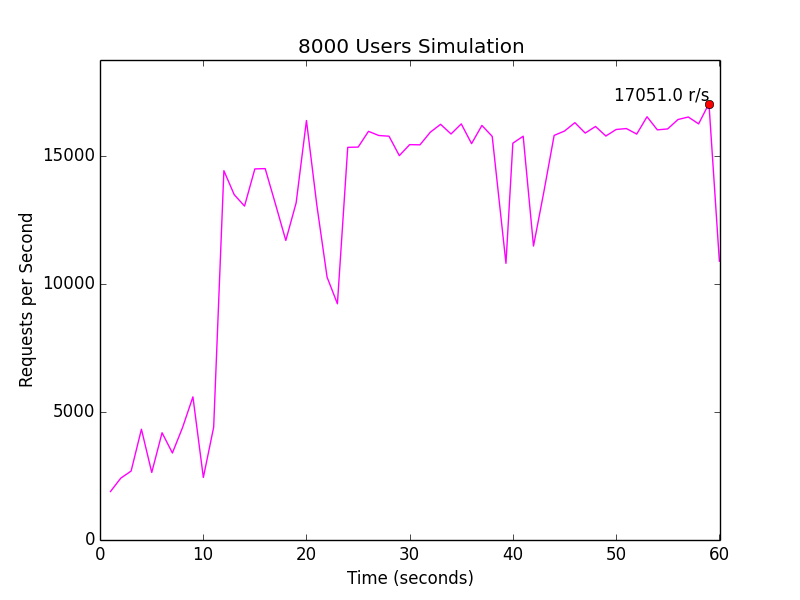
\includegraphics[scale=0.5]{diagrams/rps-8000.png}
  \caption{8000 user simulation}
  %\label{svr-struct}
\end{figure}

As you can see, the max r/s we achieved was about 17,000. This appears to be a limit of our API server. On an 8 core machine with 2000 users, we were seeing about 370\% CPU utilization. This should have been close to 800\% if we were fully parallelized. When hitting this limit, we noticed that client connections to the API server were timing out. This means the Spray-HTTP listener was not able to keep up with the connection requests or connections were being buffered. Additionally, the API server used one Actor to manage the Facebook data access. This is limiting due to how Akka messages are handled. For a future project, a different, more scalable architecture would have to be created.

%%%%%%%%%%%%%%%%%%%%%%%%%%%%%%%%%%%%%%
% Begin References
%%%%%%%%%%%%%%%%%%%%%%%%%%%%%%%%%%%%%%
\begin{thebibliography}{99}

\bibitem{sproutsocialwebsite} 
Social Media Demographics to Inform a Better Segmentation Strategy,
\\\texttt{http://sproutsocial.com/insights/new-social-media-demographics/}

\bibitem{relstatuswebsite} 
Facebook Relationship Status Statistics,
\\\texttt{http://www.statisticbrain.com/facebook-relationship-status-statistics/}

\bibitem{polstatuswebsite} 
Party Affiliation,
\\\texttt{http://www.gallup.com/poll/15370/party-affiliation.aspx}

\bibitem{interestedinwebsite} 
What percentage of the U.S. population is gay, lesbian, or bisexual?,
\\\texttt{https://www.washingtonpost.com/news/volokh-conspiracy/wp/2014/07/15/
what-percentage-of-the-u-s-population-is-gay-lesbian-or-bisexual/}

\bibitem{girlnameswebsite} 
Most Popular Girl Names in 2014,
\\\texttt{http://www.babycenter.com/popular-baby-girl-names-2014}

\bibitem{boynameswebsite} 
Most Popular Boy Names in 2014,
\\\texttt{http://www.babycenter.com/popular-baby-boy-names-2014}

\bibitem{lastnameswebsite} 
Most Popular Last Names,
\\\texttt{https://en.wikipedia.org/wiki/ListofmostcommonsurnamesinNorthAmerica}

\bibitem{fbactwebsite} 
Most popular activities of Facebook users worldwide as of 3rd quarter 2015
\\\texttt{http://www.statista.com/statistics/420714/top-facebook-activities-worldwide/}

\bibitem{randomgeneratorcontent} 
Watchout4Snakes,
\\\texttt{http://watchout4snakes.com/wo4snakes/Random/RandomPhrase}

\bibitem{fbstatswebsite} 
The Top 20 Valuable Facebook Statistics,
\\\texttt{https://zephoria.com/top-15-valuable-facebook-statistics/}

\bibitem{fbstats2website} 
When are Facebook Users Most Active?,
\\\texttt{http://mashable.com/2010/10/28/facebook-activity-study/7tNySamgEkqt}

\end{thebibliography}

\end{document}

\end{document}
